%======================================================================
\section{The project in one page}
%======================================================================

\textbf{What it does.} You give the system one photo of a face. It finds points on the
face (eye corners, nose, mouth, jaw\dots), compares the left half with the mirror image of
the right half, and reports how far the face is from perfectly mirror-symmetric. Before it
reports anything, it checks whether the photo is good enough. It answers \textbf{accept},
\textbf{caution} or \textbf{reject}, and explains why.

\textbf{Input:} one RGB photo containing a face.\\
\textbf{Output:} accept/caution/reject with reasons; a global asymmetry number $A$ (in \% of the
eye-corner distance); values for brows, eyes, nose, mouth and jaw; a stability band; pictures
(overlays); a CSV/JSON export.\\
\textbf{Constraints:} 2D image only, no model training, runs on a laptop CPU
(\runtime\,ms per image), and it is \emph{not} a medical, beauty or identity score.

\textbf{Why it is needed.} Existing tools always return a number, even for photos that cannot
support one. We found that on ordinary in-the-wild photos the measured asymmetry follows how
far the head is turned almost perfectly ($\rho$ = \rhoYawRef{}), even when the points are
placed by human experts. Without a check, a ``symmetry score'' of a selfie mostly measures
head pose.

\textbf{Our four contributions.}
\begin{enumerate}
\item \textbf{Correct pairs and a fitted mirror line.} Each point is compared with its true
anatomical twin, and the mirror line is estimated rather than assumed vertical. The older
nearest-neighbour (KD-tree) matching picks the wrong twin \kdWrong\% of the time.
\item \textbf{The mirror test.} We run the detector on the photo \emph{and} on its mirror
image. A face's asymmetry cannot change when the photo is flipped, so if the two results
disagree, the landmarks are unreliable. This needs no ground truth.
\item \textbf{A quality and pose gate} with seven signals, whose thresholds were fixed a priori
or learned on training images only.
\item \textbf{A way to evaluate without symmetry labels:} compare with the same measurement
made from expert-placed landmarks, and degrade photos in 26 controlled ways.
\end{enumerate}

\begin{center}
\begin{tabular}{@{}lc@{}}
\toprule
Headline result (LFPW test set) & Value\\
\midrule
Agreement with expert-landmark reference, baseline $\rightarrow$ ours (Spearman $\rho$) & \rhoMzero{} $\rightarrow$ \rhoMthree{}\\
Wrong partners chosen by the baseline's KD-tree matching & \kdWrong\%\\
Mirror test vs.\ true landmark error (Spearman $\rho$) & \rhoMirrorNme{}\\
Silent failures on degraded photos, no gate $\rightarrow$ full system & \silentPoolOne\% $\rightarrow$ \silentPoolThree\%\\
Score drift reduction from mirror averaging & \driftReduction\%\\
Head yaw vs.\ asymmetry, even from expert landmarks (Spearman $\rho$) & \rhoYawRef{}\\
\bottomrule
\end{tabular}
\end{center}

\begin{say}
``Existing symmetry tools always give you a number. Ours first checks whether the photo can
support a measurement, verifies its own landmarks with a mirror test, and measures with
the correct anatomical pairs and a fitted symmetry axis. We evaluated it against expert
landmarks and under 26 controlled degradations.''
\end{say}

%======================================================================
\section{Background you need}
%======================================================================

\subsection{Facial landmarks}
A \textbf{landmark} is a named point on the face, such as ``outer corner of the left eye''
or ``tip of the nose''. A \textbf{landmark detector} is a pretrained model that finds these
points in a photo.

\begin{itemize}
\item \textbf{The 68-point layout} (iBUG / 300-W) is the standard layout of academic
benchmarks: 17 jaw points, 10 eyebrow points, 9 nose points, 12 eye points and 20 mouth
points. Human experts annotated thousands of photos with it. That is why we report our
results in this layout: we can compare against the experts.
\item \textbf{MediaPipe Face Landmarker} (Google) finds 478 points, a dense mesh covering the
whole face (468 face points + 10 iris points). It runs in real time on a CPU and also outputs
a $4\times4$ \emph{transformation matrix} that tells us the head's rotation.
\item \textbf{The canonical face model} is MediaPipe's ``average face'' in 3D, with the same 468
vertices. It is \emph{exactly} left--right symmetric. We use this fact to know which vertex
is the mirror twin of which (\cref{sec:perm}).
\end{itemize}

\subsection{What ``symmetric'' means geometrically}
A face is mirror-symmetric if there is a line (the \textbf{symmetry axis} or \textbf{midline})
such that reflecting the left half across it lands exactly on the right half.
\begin{itemize}
\item \textbf{Bilateral pairs}: points that have a twin on the other side (left eye
corner $\leftrightarrow$ right eye corner).
\item \textbf{Midline points}: points that are their own twin (nose tip, chin, centre of the lips).
\item \textbf{Asymmetry}: how far a point is from where the mirror image of its twin says it
should be.
\end{itemize}

\begin{center}
\begin{tikzpicture}[scale=1.0,>=Stealth]
\draw[magenta,very thick] (0,-1.6) -- (0,1.8) node[above,black]{\small symmetry axis};
\fill[green!60!black] (-1.8,0.9) circle (2.5pt) node[left]{\small $p_i$ (left eye corner)};
\fill[black!70] (1.6,1.05) circle (2.5pt) node[right]{\small $p_{\pi(i)}$ (its twin)};
\fill[red!80!black] (-1.6,1.05) circle (2.5pt);
\draw[->,dashed,black!50] (1.55,1.05) -- (-1.5,1.05);
\node[red!80!black,above] at (-1.45,1.15) {\small reflection};
\draw[very thick,black!70] (-1.8,0.9) -- (-1.6,1.05);
\node[below] at (-1.55,0.75) {\small residual $r_i$};
\fill[black!70] (0,-0.2) circle (2.5pt) node[right]{\small midline point (nose tip)};
\end{tikzpicture}
\end{center}
The \textbf{residual} $r_i$ is the small gap between a point and the reflection of its twin.
For a perfectly symmetric face every residual is zero.

\subsection{Normalisation: why ``\% IOD''}
Distances in pixels depend on image size: a face photographed close up has bigger
gaps. We divide every distance by the \textbf{inter-ocular distance (IOD)}, the distance
between the two outer eye corners. It is the standard normaliser of the 300-W benchmark. An
asymmetry of ``2\% IOD'' means ``2\% of the distance between the outer eye corners''. On an adult face that distance is roughly 9\,cm, so
2\% IOD is just under 2\,mm.

\subsection{Head pose: yaw, pitch and roll}
\begin{itemize}
\item \textbf{Roll}: tilting the head towards a shoulder (in-plane rotation). A 2D rotation
can undo it, and our fitted axis is unaffected by it.
\item \textbf{Yaw}: turning the head left or right (shaking ``no''). One half of the face
gets foreshortened in the photo, and \emph{no 2D operation can undo that}.
\item \textbf{Pitch}: nodding up or down. It distorts vertical proportions.
\end{itemize}
This is the core limitation of any 2D symmetry measurement, and the reason the gate checks
yaw and pitch.

\subsection{Statistics used in the results}
\begin{itemize}
\item \textbf{Spearman $\rho$} (rank correlation): do two measurements put the faces in the
same order? 1 = identical order, 0 = unrelated. It works even when the two measurements use
different units, which is why we use it to compare the baseline (face-width units) with ours
(IOD units).
\item \textbf{Pearson $r$}: linear correlation.
\item \textbf{MAE} (mean absolute error): the average of $|A_{\text{ours}}-A_{\text{ref}}|$, in \% IOD.
\item \textbf{NME} (normalised mean error): the average distance between detected and
expert landmarks, divided by IOD. The standard landmark-accuracy metric.
\item \textbf{Wilcoxon test}: a paired test of whether one measurement is systematically
larger than another.
\end{itemize}

%======================================================================
\section{The baseline we improve on (M0)}
%======================================================================
The closest public tool is \texttt{nashokan/FacialAsymmetry} on GitHub. It implements the
symmetry part of Varghaei et al.\ (ICCV Workshops 2025). Since the repository has \textbf{no
licence}, we did not copy its code; we \textbf{re-implemented its method} from its description.
Its steps are:
\begin{enumerate}
\item Detect the 478 MediaPipe points.
\item Align the face: rotate and scale the image so that vertices 33 and 263 sit at fixed
positions, then detect again.
\item Take a vertical midline at the average $x$ of vertices 33 and 263.
\item Reflect every point on the left of the midline, and match it to the \emph{nearest}
right-side point (KD-tree nearest-neighbour search).
\item Report the mean matched distance divided by face width.
\end{enumerate}

\textbf{Its three problems, which we measured:}
\begin{enumerate}
\item \textbf{Wrong partners.} The mesh is dense, so the nearest point after reflection is
often a \emph{neighbour} of the true twin. The matching then absorbs part of the asymmetry it
should measure. On LFPW, \kdWrong\% of matches are the wrong anatomical twin
(\cref{fig:corr}).
\item \textbf{Assumed vertical midline.} Any tilt of the head, or any error in vertices 33/263,
looks like asymmetry. Without the alignment step the baseline's agreement drops from
\rhoMzero{} to \rhoMzeroNoAlign{}.
\item \textbf{No quality check.} It always returns a number.
\end{enumerate}
(Detail worth knowing: vertices 33 and 263 are the \emph{outer} eye corners, although the
baseline's code comments call them inner corners.)

\begin{figure}[h]
\centering
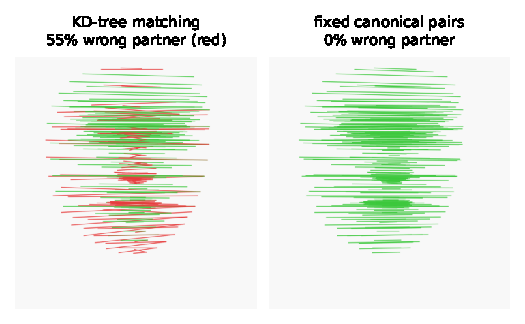
\includegraphics[width=0.6\linewidth]{correspondence.pdf}
\caption{Matches for one face (geometry only). Left: KD-tree matching; red lines are wrong
partners. Right: our fixed anatomical pairs.}
\label{fig:corr}
\end{figure}
